


\begin{minipage}{\linewidth}
\begin{center}
\includegraphics[width=.95\columnwidth]{graphics/LineSegmentDelta.pdf}
\captionof{figure}{}\label{fig:LineSegmentDelta.pdf}
\end{center}
\end{minipage}
\begin{eqnarray*}
\sin \lr{\frac{\pi}{6} - \chi} &=& \frac{1}{2+\psi}\\
\sin \frac{\pi}{6} \cos \chi &=& \frac{1}{2+\psi} + \cos \frac{\pi}{6} \sin \chi\\
&\iff&\\
\frac{1}{2} &\geq& \frac{1}{2} \cos \chi \\
&=& \frac{1}{2+\psi} + \frac{\sqrt{3}}{2} \sin \chi\\
&\geq& \frac{1}{2+\psi} + \frac{\sqrt{3}}{2} \lr{ \chi - \frac{\chi^3}{6}}\\
&\iff&\\
\frac{1}{2}-\frac{1}{2+\psi} &\geq& \frac{\sqrt{3}}{2} \lr{ \chi - \frac{\chi^3}{6}} \qquad \text{if }\chi < 1\\
\frac{\psi}{2 ( 2 + \psi)} &\geq&  \frac{5\sqrt{3}}{12} \chi\\
\frac{3 \psi}{5\sqrt{3}}=\frac{12}{5\sqrt{3}} \frac{\psi}{4} &\geq& \chi
\end{eqnarray*}

\begin{minipage}{\linewidth}
\begin{center}
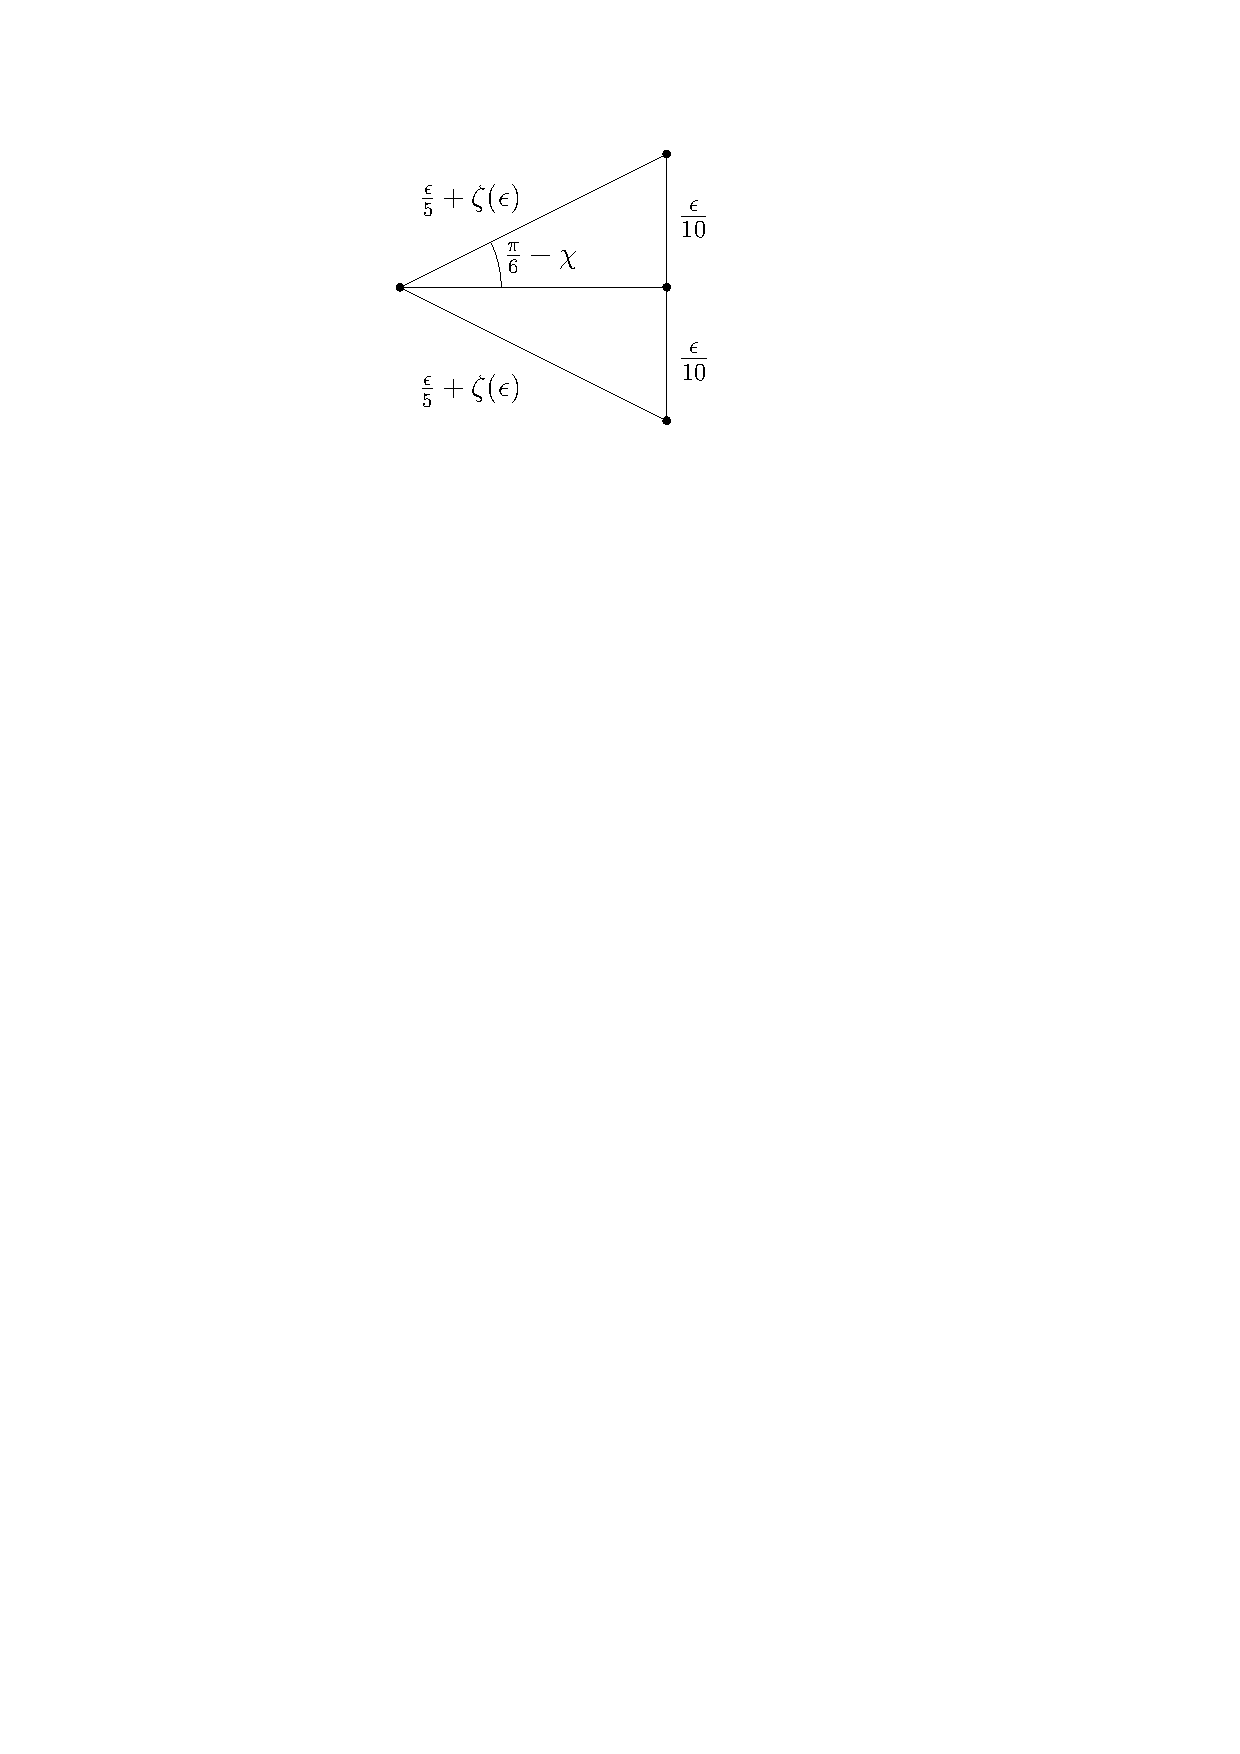
\includegraphics[width=.20\columnwidth]{graphics/part1ch4.pdf}
\captionof{figure}{}\label{fig:part1ch4.pdf}
\end{center}
\end{minipage}
\begin{eqnarray*}
\sin \lr{\frac{\pi}{6}- \chi} &=& \frac{1}{2+ \psi}\\
\sin \frac{\pi}{6} \cos \chi - \cos \frac{\pi}{6} \sin \chi &=& = \frac{1}{2+\psi}\\
\frac{1}{2} \cos \chi - \frac{\sqrt{3}}{2} \sin \chi &=& \frac{1}{2+\psi}\\
&\geq& \frac{1}{2+\psi} + \frac{\sqrt{3}}{2} \chi - \frac{\sqrt{3}}{12} \chi^3 \\
\frac{1}{2} &\geq&  \frac{1}{2+\psi} + \frac{\sqrt{3}}{4} \chi\\
\end{eqnarray*}

$$\frac{\psi}{4} \geq \frac{\psi}{2 (2 + \psi)}\geq \frac{\sqrt{3}}{4} \chi\iff \frac{\psi}{\sqrt{3}} \geq \chi$$

$$\frac{\pi}{3} - 2 \chi = \lambda_\text{min} \leq \lambda \leq \lambda_\text{max} = \frac{\pi}{3} + 10 \chi$$


\begin{minipage}{\linewidth}
\begin{center}
\includegraphics[width=.66\columnwidth]{graphics/ch4Paralellogram.pdf}
\captionof{figure}{}\label{fig:ch4Paralellogram.pdf}
\end{center}
\end{minipage}